A partir do livro de engenharia do Prof. Ogata \cite{ogata2003}, estou desenvolvendo a revisão bibliografica dos sistemas de controle para inicio do projeto PID.\\
Para o projeto do atuador PID, será seguido o fluxograma de projeto abaixo onde cada caixa corresponderá a um esforço de projeto.\\
Inicialmente com recursos computacionais, como Matlab, serão feitas simulações para que se estabeleçam os melhores parâmetros de sensoriamento e atuação.\\
Estando os mesmos de acordo os componentes de mercado e de acordo aos equipamentos onde será instalado o sistema, passará a ser montado um protótipo.\\
\justifying
%\centering
	\begin{figure}
		\centering
		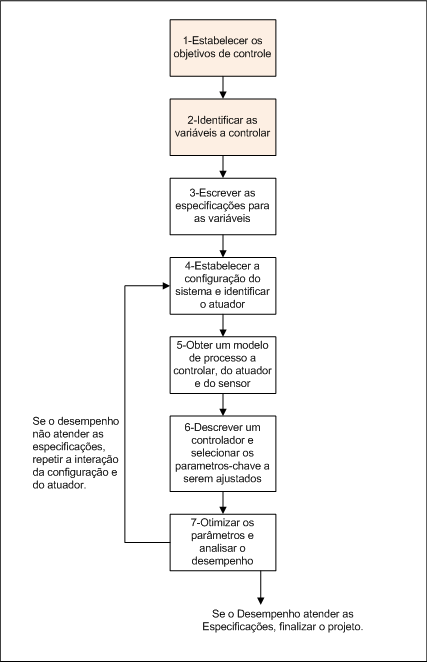
\includegraphics[width=0.7\linewidth]{./ima/fluxo1.png}
		%\caption{}
		\label{fig:fluxo1}
		\caption{Organograma de Projeto}
	\end{figure}
	
Conforme o fluxograma do projeto, os itens 1 e 2 já estão em desenvolvimento e para próxima semana será mais especificado cada um deles. \\
